%; whizzy chapter
% -initex iniptex -latex platex -format platex -bibtex jbibtex -fmt fmt
% 以上 whizzytex を使用する場合の設定。


%     Tokyo Debian Meeting resources
%     Copyright (C) 2009 Junichi Uekawa

%     This program is free software; you can redistribute it and/or modify
%     it under the terms of the GNU General Public License as published by
%     the Free Software Foundation; either version 2 of the License, or
%     (at your option) any later version.

%     This program is distributed in the hope that it will be useful,
%     but WITHOUT ANY WARRANTY; without even the implied warranty of
%     MERCHANTABILITY or FITNESS FOR A PARTICULAR PURPOSE.  See the
%     GNU General Public License for more details.

%     You should have received a copy of the GNU General Public License
%     along with this program; if not, write to the Free Software
%     Foundation, Inc., 51 Franklin St, Fifth Floor, Boston, MA  02110-1301 USA

%  preview (shell-command (concat "evince " (replace-regexp-in-string "tex$" "pdf"(buffer-file-name)) "&"))
% 画像ファイルを処理するためにはebbを利用してboundingboxを作成。
%(shell-command "cd image200901; ebb *.png")

%%ここからヘッダ開始。

\documentclass[mingoth,a4paper]{jsarticle}
\usepackage{monthlyreport}

% 日付を定義する、毎月変わります。
\newcommand{\debmtgyear}{2009}
\newcommand{\debmtgmonth}{1}
\newcommand{\debmtgdate}{17}
\newcommand{\debmtgnumber}{48}



\begin{document}

\begin{titlepage}
\thispagestyle{empty}

% タイトルページ:編集必要な部分は最初のマクロに飛ばすこと

\vspace*{-2cm}
第\debmtgnumber{}回 東京エリア Debian 勉強会資料

\hspace*{-2.4cm}
\includegraphics[width=210mm]{image200801/2008title.eps}\\
\hfill{}\debmtgyear{}年\debmtgmonth{}月\debmtgdate{}日

\end{titlepage}

\dancersection{Introduction}{上川 純一}

\begin{multicols}{2}
 
 
 今月のDebian勉強会へようこそ。これからDebianの世界にあしを踏み入れると
 いう方も、すでにどっぷりとつかっているという方も、月に一回Debianについ
 て語りませんか?

 Debian勉強会の目的は下記です。

 \begin{itemize}
 \item \underline{Debian Developer} (開発者)の育成。
 \item 日本語での「\underline{開発に関する情報}」を整理してまとめ、アップデートする。
 \item \underline{場}の提供。
 \begin{itemize}
  \item 普段ばらばらな場所にいる人々が face-to-face で出会える場を提供
	する。
  \item Debian のためになることを語る場を提供する。
  \item Debianについて語る場を提供する。
 \end{itemize}
 \end{itemize}		

 Debianの勉強会ということで究極的には参加者全員がDebian Packageをがりがり
 と作るスーパーハッカーになった姿を妄想しています。情報の共有・活用を通し
 て Debianの今後の能動的な展開への土台として、「場」としての空間を提供す
 るのが目的です。

 2009年の計画は仮です。

 \begin{enumerate}
  \item 新年の企画 (アンサンブル荻窪開催)
  \item OSC
  \item (東京大学?)
  \item (千代田区都立図書館?\footnote{\url{http://www.library.chiyoda.tokyo.jp/}})
  \item (東京大学?)
  \item 
  \item スペインにて開催
  \item Debconf報告会
  \item 
  \item 
  \item 
  \item 忘年会
 \end{enumerate}

 会場候補としては下記があります:

 \begin{itemize}
  \item 大学
  \item 恵比寿SGIホール
  \item Googleオフィス
  \item 公民館(あんさんぶる荻窪等)
  \item 都立会議室(無線LAN)
  \item 健保の施設
 \end{itemize}

\end{multicols}


\newpage

\begin{minipage}[b]{0.2\hsize}
 \definecolor{titleback}{gray}{0.9}
 \colorbox{titleback}{\rotatebox{90}{\fontsize{80}{80} {\gt デビアン勉強会} }}
\end{minipage}
\begin{minipage}[b]{0.8\hsize}
\hrule
\vspace{2mm}
\hrule
%
% there are too many entries in 200901, usually
% we have tocdepth=2.
%
\setcounter{tocdepth}{1}
\tableofcontents
\vspace{2mm}
\hrule
\end{minipage}

\dancersection{事前課題}{上川 純一}


2012年の正月、僕は実家に帰って旧友を深めるべく喫茶店にいた。最近ここら
へんには立ち寄っていないなぁ。そういうことをつらつらと思っているとふと
人影が目に入る。

「おぉ、待たせたな」

「あぁ。久しぶり」

「どうした」

「いや」

そして僕は手元のDebianデバイスから目をはなす。

「お、Debianの調子はどうよ、最近はどんな使い方しているの?」

この質問をいま僕にするなんて。血圧がすこし上がるのを感じながら
僕は饒舌になりすぎないように説明する。

「(A)」


{\bf 問題}

\begin{enumerate}
 \item Debianに関しての、2009年の抱負を述べよ
 \item 「2012のDebian」と題して(A)を埋めよ
\end{enumerate}

この課題に対して提出いただいた内容は以下です。

\begin{multicols}{2}
 %; whizzy-master ../debianmeetingresume200901.tex
% $B0J>e$N@_Dj$r$7$F$$$k$?$a!"$3$N%U%!%$%k$G(B M-x whizzytex $B$9$k$H!"(Bwhizzytex$B$,MxMQ$G$-$^$9!#(B

\begin{prework}{$B>e@n=c0l(B}
\preworksection{Debian$B$K4X$7$F$N!"(B2009$BG/$NJzIi(B}

\begin{itemize}
 \item $B;H$C$F$$$k%Q%C%1!<%8$r%a%s%F%J%s%9!";H$C$F$J$$%Q%C%1!<%8$r<N$F$k(B
 \item $B:#;_$^$C$F$$$k(B pbuilder / cowdancer / qemubuilder $B$N%j%0%l%C%7%g%s%F%9%H%5!<%P$r(B
       $BI|3h$5$;$k(B
\end{itemize}

\preworksection{2012$B$N(BDebian}

$B;~7W$J$s$@$1$I$5!"%?%C%A%9%/%j!<%s$H%W%m%8%'%/%?$,$D$$$F$$$F!"$=$l$GF0$/(B
$B$s$@$<!#(B

\end{prework}

\begin{prework}{$B;3K\(B $B9@G7(B}
\preworksection{Debian$B$K4X$7$F$N!"(B2009$BG/$NJzIi(B}

$B%a%s%F%J%s%9$7$F$$$k%Q%C%1!<%8$rCOL#$KA}$d$7$F$$$/!#(B

\preworksection{2012$B$N(BDebian}

$B=gD4$K(B squeeze $B$N%j%j!<%9$bCY$l$F$^$9$J!#(B

\end{prework}


\begin{prework}{$B4d>>(B $B?.MN(B}
\preworksection{Debian$B$K4X$7$F$N!"(B2009$BG/$NJzIi(B}
\begin{itemize}
\item DD $B$K$J$k!#(B
\item $BB>$N%5%V%W%m%8%'%/%H$K$b@Q6KE*$K;22C$9$k!#(B
\item SH $B$N3+H/$r7QB3$9$k!#(B
\end{itemize}

\preworksection{2012$B$N(BDebian}

$B$^$@L\$GA`:n$9$k$N$O47$l$J$$$J!#%a%,%M$GA`:n$9$k$N$O$D$i$$$<!#(B

\end{prework}

% $B$3$N>e$NItJ,$K0J2<$NFbMF$rA^F~$9$k!#(B
% \begin{prework}{$BL>A0(B}
% \preworksection{XXX}
% \preworksection{YYY}
% \end{prework}
%

\end{multicols}

% image200901/prework.tex 内部にテキストを追加してください。
%
%


\dancersection{最近のDebian関連のミーティング報告}{上川 純一}
\subsection{東京エリアDebian勉強会47回目報告}
% (query-replace-regexp "<.*?>" "")
% (query-replace-regexp "^[	 ]\+" "")

東京エリアDebian勉強会報告。
2008年12月20日土曜日に第47回東京エリアDebian勉強会を実施しました。
今回の参加者は
前田耕平さん、
一井崇さん、
やまだたくまさん、
小室文さん、
平澤俊雄さん、
藤沢理聡さん、
じつかたさん、
岩松信洋さん、
小林儀匡さん、
山本浩之さん、
キタハラさん、
日比野啓さん、
id774さん、
やまねひできさん、
でんさん、
でんさんの友人Aさん、
上川x2の
18名でした。

まず、2008年の勉強会の実績について上川が話をしました。
今回まとめてみた情報は、参加人数と事前課題の提出実績と
事後のブログ掲載の率です。
事後のブログ掲載は開催している側としては励みになるのでうれしい
というような話をした気がします。


次に上川が、2009年にむけて最近のトレンドについて
整理して、SWOTの図を作成するという企画をしました。
議論はいろいろと発散しましたが、アクションアイテムはたくさんでてきたので
これが次につながるとよいですね。


最後にライトニングトークを実施しました。
小林さんは apt-cache dotty の話。
id774さんはDebianユーザとしての告白。
上川は sqlite3 使って見ましたネタ。
やまだたくまさんは資料の翻訳のやりかたについて、機械翻訳をベースにどう労力を節約するかというネタ。
岩松さんは日本 . ユーザ会設立について。
前田さんはヨメをDebianユーザにする方法。
日比野さんはocamlユーザ会設立宣言。

\subsection{Debian JP 定例会議 on IAX}

Debian JP の定例会議は通常 IRC で行っているのですが、2009年1月8日に執り行
われた会議は実験的に音声通話も交えて行いました。利用したプロトコルはIAXプ
ロトコルで、iaxcomm をクライアントとして利用し、asterisk サーバに全員接続
しました。

MacBookのマイクまわりのハックが十分でなく、iaxcomm 自体の安定度合いもよく
なかったので音質が悪いという問題がありましたが通信状態は概ね良好でした。
今後さらに試験を重ねて実用的に使って行きたいものです。


% ===============================================================
\dancersection{Git+メールでの事前課題提出にまつわる課題}{上川純一}
\index{git}
% ===============================================================

2008年11月、12月、および2009年1月には事前課題をGitを利用してGitの生成する
パッチをメールで提出してもらうという形式にしていました。
その場合には git pull するたびにコンフリクトが発生します。
その原因となる仕組みと対策方法について説明します。

\subsection{コンフリクトが発生しやすい理由}

それでは、Debian 勉強会の2008年11,12月の資料でコンフリクトが発生しやすかっ
た理由を分析してみましょう。

\subsubsection{元のファイルの形式}

\begin{commandline}
-\subsection{}
+\subsection{XXXX}
+内容
+
\end{commandline}

同じファイルについて作業し、しかも同じ場所にすこしづつ異なる変更を別の人
が行うという仕組みになっていました。この場合、二つのパッチはかならずコン
フリクトし、手動で解消する必要があります。今回パッチが同じ場所に挿入して
いる場合に、順序は問わないので適当でよいのですが、\texttt{git apply} には
その知識はないため、毎回コンフリクトの解消を行います。

\subsubsection{メールを利用したサブミット}

\begin{figure}
 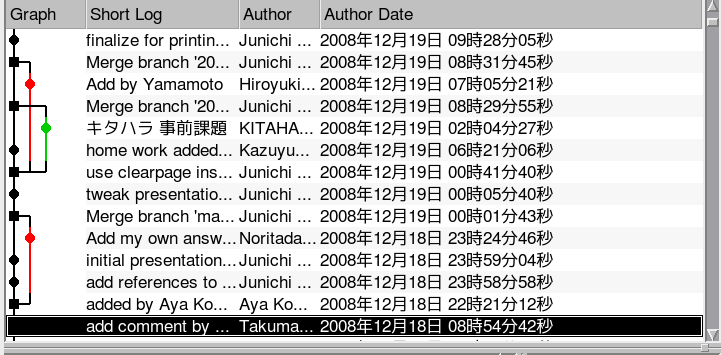
\includegraphics[width=\hsize]{image200901/qgit-trees.png}
 \caption{qgitでみたツリーの状況、手動でマージが複数発生している}
 \label{fig:mergedtokyodebian}
\end{figure}

締切り直前に作業するのが習慣のため、
複数の人がある時点の同じコミットに対してパッチを作成、
それを上川がある時点でマージしました(\fgref{fig:mergedtokyodebian})。

毎回コンフリクトが発生するのですが、それを上川が解消してマージとして記録
されています。そのため、各自が提出したバージョンとは若干違うパッチとなっ
てalioth.debian.orgにあるGitツリーにマージされています。

\subsection{マージ・コンフリクトの発生のしかた}

Gitはデフォルトではmasterブランチで作業します。\texttt{git pull} コマンドはAlioth
にあるリモートのツリーの情報をoriginブランチにとってきて、masterブランチ
にマージします。マージする内容がなければ、Fast-forward されます。

まず最初に各自が自分のGitツリーの master ブランチでパッチを作成します。そ
して、\texttt{git format-patch} の結果をパッチファイルとして送付します。上川が
\texttt{git am} でそのパッチを適用し、Alioth のGitツリーに公開します。複数人が同時
期に事前課題を提出しているため、\texttt{git am} でパッチを適用した場合にそのままで
は適用できない状況がおき、「コンフリクト」が発生します。「コンフリクト」
が発生した場合には上川が手動でその部分を修正します。

各自がAliothのGitツリーの最新バージョンを \texttt{git pull} で取得してくると
origin ブランチには上川の作成した変更を伴ったパッチが入ります。
masterブランチで自分の作成したものからは若干変更が加わっています。
そのため、内容に整合性がとれるとはかぎらないため、コンフリクトが発生しま
す。コンフリクトがおきなかったとしても履歴にマージが残ります。

\subsection{マージ・コンフリクトの解消方法}

\subsubsection{rebase して履歴をきれいにする}

マージなどを解消するためには、\texttt{git rebase -i origin} で不要なパッチを目視し
て消す作業をすればよいです。そもそも \texttt{git pull --rebase} すると、おそらくマー
ジが残らないが、コンフリクトの解消は必要になります。これは面倒です。

\subsubsection{作業の仕方を変える}

解決策としては、各自が提出用のブランチを作成してそこで作業し、そこで提出
用のデータを作成してしまえばよいというのがあります。

\begin{commandline}
 
$ git checkout -b preworkXXXX origin
$ # ... このブランチで作業
$ git format-patch ... 

# 提出してしまったらmasterブランチにもどる
$ git checkout master 
$ git pull # 上川の適用した版がとりこまれる

# さらに新しいブランチを作成して次の月の作業を行う
$ git checkout -b preworkYYYY origin
\end{commandline}

preworkXXXX ブランチを毎回捨てる。

\subsubsection{format-patchではない方法を使う}

もう一つの選択肢としては、format-patchではない方法でデータの送受信を行う
ことがあります。
format-patchと git am の送受信の過程でコミットのハッシュが異なっているこ
とから各位のコンフリクトが発生しているのだろうということです。

git bundle でバイナリ形式でデータを送付することができます。これを使うとハッ
シュは保存されるので上川のコンフリクトは解消されませんが、コンフリクトを
解消したログがそのまま残るので、各位のコンフリクトは発生しないでしょう。

\subsection{リポジトリ管理者側の課題}

視点をすこし変えてリポジトリの管理者として上川の作業を見てみましょう。
git am でパッチを適用して、マージするという作業を行うのですが、そのワー
クフローは実は面倒です。

特にメールを受けて、git am がコンフリクトを起こす確率が高く、
複数のパッチがあるとほぼ確実にコンフリクトを解消することになります。

現状は複数の一時的に利用するブランチに git am で適用したものをあとでマー
ジする、という方法をとっています。

\begin{commandline}
  git checkout -b マージ用のブランチA master
  git am -3 パッチ
  git checkout -b マージ用のブランチB master
  git am -3 パッチ
  git checkout master 
  git merge マージ用のブランチA マージ用のブランチB
  コンフリクトの解消
  git commit -a 
\end{commandline}

ただ、10人以上の事前課題のハンドリングには時間もかかり、毎回したい作業
ではないです。

自動でコンフリクトするかしないかについては判定できるし、その結果がビルド
するかはチェックできるのであれば、自動処理でコミットを管理できないか?と考
えています。

最低限のチェックだけしてパッチを master ブランチに自動でとりこんでくれる
ような仕組み、ないもんでしょうかねぇ?

%============================================================
\dancersection{NamazuみたいにGoogle AJAX Search API}{小室 文}
\index{Google AJAX Search API}
\index{javascript}
\index{search}
%============================================================

自分のウェブサイトの検索用にわざわざNamazuを導入しなくても
Googleの検索エンジンを使ってお手軽にサイト内全文検索する方法を説明します。

\subsection{Googleの検索エンジンをカスタマイズして使うには}

利用するパターンがいくつかあります。それぞれのパターンについて設定方法を
紹介します。

どれを選んでも基本はHTMLファイル(もしくはPHPなど)をウェブサーバに置くことで動
作します。JavaScript版はブラウザさえあればどこでも動きます。

\begin{enumerate}
\item JavaScriptあり
\begin{enumerate}
\item 自分でJavaScriptを組む
\item ウィザードを使う
\end{enumerate}
\item JavaScriptなし
\end{enumerate}


\subsubsection{JavaScriptあり・なし両方}
Google AJAX Search APIのKEYを事前に取得しておきます。

\subsubsection{JavaScriptあり}
HTMLファイルの中で Google AJAX Search API JavaScript ライブラリをロード
します。
\begin{commandline}
<script src="http://www.google.com/uds/api?file=uds.js&v=1.0" type="text/javascript"></script>
\end{commandline}
\begin{commandline}
//名前空間の為に追加
    google.load("search", "1.0"); 

//検索をするオブジェクトを作成する
    var searchControl = new google.search.SearchControl(); 

//検索準備
//子オブジェクトのサーチャーメソッドを検索コントロールに追加。必要であればオプションも。 
    var options = new GsearcherOptions(); //表示オプション指定
    options.setExpandMode(GSearchControl.EXPAND_MODE_OPEN);//結果一覧を開いた状態で出力する
    options.setExpandMode(GSearchControl.EXPAND_MODE_CLOSED);//結果を閉じた状態のまま結果出力をする
    options.setExpandMode(GSearchControl.EXPAND_MODE_PARTIAL);//結果がオープン拡張モード
    options.setRoot(document.getElementById("resultsComeHere"));//結果を指定する場所に表示するオプション

//サイト制限の設定
    var siteSearch = new GwebSearch();
    siteSearch.setUserDefinedLabel("Aya's Site");
    siteSearch.setSiteRestriction("popowa.com");//直接URLを指定
    siteSearch.setSiteRestriction("000455696194071821846:reviews");//カ
 スタムエンジンのKeyを指定\footnote{カスタム検索エンジンとはウィザードで
 検索窓をある程度のデザインや制限を付けて作ることが出来るものです。\\
\url{http://www.google.com/coop/cse/}}

//準備終了、セットする
    searchControl.addSearcher(siteSearch, options);//オプションがあれば
    searchControl.addSearcher(new GwebSearch());//オプションがなければ
//出力準備
    var result = document.getElementById("googleResults");
    var drawOptions = new GdrawOptions();//オプション用にdrawOptions オブジェクトを作成
    drawOptions.setDrawMode(GSearchControl.DRAW_MODE_LINEAR);//1)一列に出力
    drawOptions.setDrawMode(GSearchControl.DRAW_MODE_TABBED);//2)タブに出力
    drawOptions.setSearchFormRoot(document.getElementById("searchForm"));//検索結果と検索フォームを切り離す機能
    searchControl.draw(result, drawOptions);
//検索結果の保持(prototype)
    searchControl.setOnKeepCallback(this, MyKeepHandler);//この(this)検索状況をMyKeepHandlerに持たせておく。
    searchControl.setSearchCompleteCallback(this, OnSearchComplete); //検索の実行後
    searchControl.setSearchStartingCallback(this, OnSearchStarting); //検索の完了前
//検索する!
    searchControl.execute(keyword);
\end{commandline}
そして、body内に検索窓、検索結果を出力したい場所にdivを入れます。
\begin{commandline}
 <div id="searchForm" class="searchForm">form</div>
 <div id="googleResults" class="googleResults">googleResults</div>
\end{commandline}


\subsubsection{JavaScriptなし}
\url{http://ajax.googleapis.com/ajax/services/search/web}
に引数を渡してリクエストするとJSON形式でレスポンスが得られます。

\begin{table}[h]
\begin{tabular}{|l|l|l|}
\hline
パラメータ & 項目 & 注意事項 \\
\hline
   q? & 検索したいキーワード、検索式 & 日本語だった場合はurlencode()しないとうまく動かない\\
\hline
   v=1.0 & プロトコル番号の指定 & 現在は1.0しかない\\
\hline
   key? & Google AJAX Search APIのKey & 申請したFQDN=実際に使っているFQDNでなくてもよい\\
\hline
   start? & 検索結果の開始インデックス & ドメイン指定をすると160件から持って来てくれなくなる\\
\hline
   cx? & カスタム検索エンジンのID & 特定のドメインからのみ検索する事が出来る\\
\hline
   lr? & 特定の言語のドキュメントを検索対象とする & \\
\hline
\end{tabular}
\end{table}
レスポンス形式
\begin{commandline}
{"responseData": {
 "results": [
  {
   "GsearchResultClass": "GwebSearch",
   "unescapedUrl": "http://en.wikipedia.org/wiki/Paris_Hilton",
   "url": "http://en.wikipedia.org/wiki/Paris_Hilton",
   "visibleUrl": "en.wikipedia.org",
   "cacheUrl": "http://www.google.com/search?q\u003dcache:TwrPfhd22hYJ:en.wikipedia.org",
   "title": "\u003cb\u003eParis Hilton\u003c/b\u003e - Wikipedia, the free encyclopedia",
   "titleNoFormatting": "Paris Hilton - Wikipedia, the free encyclopedia",
   "content": "\[1\] In 2006, she released her debut album..."
  },
  ...
 ],
 "cursor": {
  "pages": [
   { "start": "0", "label": 1 },
   { "start": "4", "label": 2 },
   { "start": "8", "label": 3 },
   { "start": "12","label": 4 }
  ],
  "estimatedResultCount": "59600000",
  "currentPageIndex": 0,
  "moreResultsUrl": "http://www.google.com/search?oe\u003dutf8\u0026ie\u003dutf8..."
 }
}
, "responseDetails": null, "responseStatus": 200}
\end{commandline}
レスポンスを個々のプログラムで処理する
\begin{commandline}
<?php
function search($keyword, $page, $key){
	$uri = 'http://ajax.googleapis.com/ajax/services/search/web';
	$uri .= '?q=' . urlencode($keyword);
	$uri .= '&key='.$key;
	$uri .= '&v=1.0&rsz=large&hl=ja&start=' . $page;
	return json_decode(file_get_contents($uri));
}
$keyword = "東京エリアDebian勉強会";
$key = 'アプリケーションのキー';
$data = search($keyword, 1, $key);
var_dump($data);
?>

\end{commandline}

\subsubsection{現状の問題点}

Google AJAX Search APIのかえしてくる「検索結果」の総数には問題があります。

JavaScriptあり:
setSiteRestrictionでドメインを指定して検索をしようとした
場合、検索結果の総数が検索するたびに変わります。

JavaScriptなし:
\verb!?q=DMC\%20site:http://www.debian.or.jp/!とするとドメイン検索は出来
るが、
\verb!start?!で引数を渡すたびに同じように結果総数が変わります。

\subsubsection{まとめ}

Namazuみたいにページ分けされた検索の仕組みは構築出来ませんでした(2009/1
現時点)。

Google AJAX Search APIの総数が変わる件については、estimatedResultCount
というくらいなので、estimateなのでしょう。
\footnote{\url{http://www.google.com/support/webmasters/bin/answer.py?hl=en&answer=70920}
'How does Google calculate the number of results?'に記述があります}
ちなみにYahoo Web検索でも同じような問題が発生します。
Yahoo!は検索リクエストがある度に検索結果を積算しているので違います、
と予め免責してあります。
\footnote{表示件数について :
\url{http://help.yahoo.co.jp/help/jp/search/web/web-14.html}}

% ===============================================================
\dancersection{AspireOneでDebian sidサーバー}{id774}
\index{AspireOne}
\index{sid}
\index{NetBook}
% ===============================================================

この冬休みを利用してAspireOneにDebian sidの環境を構築しました。
AspireOneと言えば今流行りのNetBookとしてモバイル用途で知られています。
今回はその省電力性に注目し、モバイル以外にもポータブルで場所を取らない
簡易サーバーとして利用可能なのではないかと考えトライしました。

\subsection{AspireOneでsidを使ってみる}

\subsubsection{AspireOneの電力消費効率}

\index{Atom}
AspireOneは省電力性に優れるIntel Atom CPUを搭載しており、アイドル状態
で約10W、高負荷状態でも15W程度で動作します。
高性能を要するエンコードやリッピングではなく、ちょっとしたWebサーバー等
の用途であれば安価でエコなサーバーとして利用できそうです。

\subsubsection{sidを選択する理由}

通常、サーバーであれば安定版を選択します。しかしAspireOneならいつでも
携帯して持ち運び、管理者が対話的に操作してメンテナンスすることができるの
で、これなら最新のパッケージを利用できるsidを使っても、
何かトラブルがあればすぐ対応できるでしょう。

\subsection{Debianをインストール}

Debian Wiki \footnote{\url{http://wiki.debian.org/DebianAcerOne}} に
情報がまとまっているので、基本的にこれを参考に作業しました。

\subsubsection{名刺サイズのイメージからのインストール}

sidのインストールには主に2種類の方法
\footnote{\url{http://www.debian.org/CD/faq/\#unstable-images}} があります。
\begin{itemize}
 \item テスト版のDebianのsources.listをsidに書き換えてaptitude full-upgradeする。
 \item 最小サイズの最新ビルドイメージを利用してエキスパートモードでネットワークインストールをおこなう。
\end{itemize}

今回は後者の方法を採用しました。
インストールにはDailyビルド最新版のDebianイメージ 
\footnote{\url{http://cdimage.debian.org/cdimage/daily-builds/daily/arch-latest/i386/iso-cd/}} 
を利用します。
名刺サイズのインストールイメージを利用して、エキスパートモードでインストー
ルを開始すると、不安定版を選択することができます。

\subsubsection{暗号化LVMの設定}

モバイルで外に持ち出すことを考えると、HDDやPC本体の盗難によるリスクを考
慮しなければなりません。Debianはetchから暗号化LVMを標準で利用出来るよう
になりました。これで/boot以外の領域を暗号化することができますのでセキュ
リティとしては非常に強力になるでしょう。

この際、元のWindows領域を全て上書き末梢するので4〜5時間程度かかります。
そこで一晩放置して翌日作業をするようにしました。

\subsubsection{無線LANの設定}

AspireOneにはAtheros AR5007チップが搭載されています。そこでmodule-assistantを
利用してMadWifiをインストールしました。

\begin{commandline}
sudo aptitude install build-essential module-assistant madwifi-source
sudo m-a prepare
sudo m-a auto-install madwifi
\end{commandline}

\subsubsection{イー・モバイルの設定}

現時点でlenny/sidに搭載されているカーネル2.6.26ならイー・モバイルによる通信が可
能で、さらにUSBの着脱によるプラグアンドプレイにも対応しています。

\texttt{pppconfig} パッケージをインストールし \texttt{/etc/ppp/peers/em}
ファイルに以下のように記述します。文字列はイー・モバイル固有ですのでこのまま指定します。
\texttt{dip} グループに所属したアカウントなら \texttt{pon em} コマンドを発行すれば
イー・モバイルによるネットワーク接続ができるようになります。

\begin{commandline}
user "em@em"
connect "/usr/sbin/chat -v -f /etc/chatscripts/pap -T *99***1#"
/dev/ttyUSB0
115200
noipdefault
usepeerdns
defaultroute
persist
noauth
\end{commandline}

\subsection{sidをメンテナンスする}

\subsubsection{アップグレード}

私は以下のコマンドの実行結果を \texttt{cron} で定期的に取得しています。

\begin{commandline}
aptitude update && aptitude -s -v -y full-upgrade
\end{commandline}

実際にアップグレードはしませんが更新予定のパッケージの一覧を見ることがで
きます。これに加え必要に応じて \texttt{apt-listchanges} や
\texttt{apt-listbugs} 等を使い、
既存パッケージの依存関係に影響を及ぼさないことを確認の上でアップグレード
することにしています。

\subsubsection{仮想環境での事前検証}

さらに確実性を高めるための方法としてVMwareなど仮想環境を利用する方法が
あります。あらかじめゲストOSとして実機と同じパッケージ構成のsidを用意し、
先にそちらを変更して問題が無いことを確認してから実機のパッケージを変更す
ればトラブルを避けることができます。

\subsection{まとめ}

Debian sidなら最新のドライバや機能が使えるので、流行のNetBookに
インストールしてモバイルなサーバーとして活用するのも良いですね。
ぜひみなさんもトライしてみてください。

%============================================================
\dancersection{Debian GNU/Linux 2ch ブラウザ普及計画}{山本 浩之}
\index{2ch browser}
%============================================================

結構前から色んな 2ch ブラウザを stable 用にバックポートして、2ちゃんねる
スレッドテンプレなどで非公式に upload していました。
しかし、最近 JD が公式パッケージ入りしましたが、それ以外はなかなか公式に
は入ってきてはいません。
そこでいくつかの 2ch ブラウザについて、公式パッケージ入りを検討してみました。

今回検討対象とした 2ch ブラウザは
 Navi2ch for Emacs、
\index{navi2ch}
 おちゅ〜しゃ、
\index{おちゅーしゃ@おちゅ〜しゃ}
 Kita、
\index{kita}
 Kita2、
\index{kita2}
 Chalice for Vim、
\index{Chalice}
 w3m-2ch、
\index{w3m-2ch}
 Gnview
\index{Gnview}
です、それではそれぞれみてみましょう。

% 2chブラウザの一覧を簡単に記述するためのマクロ
\newcommand{\yamamotobrowserlist}[2]{%
\begin{tabular}{|p{30zw}|p{20zw}|}
\hline 
#2 & #1\\
\hline 
\end{tabular}
}

\subsection{Navi2ch for Emacs}

\yamamotobrowserlist{ライセンス:GPL}%
{Emacs 上で動く 2ch ブラウザ。}

昔からDebian Developer の
野首さんが、Navi2ch の本家で最新の CVS 版のパッケージを配っていることで有名です。
ライセンス的にも問題はありませんが、どうやら野首さんのポリシーとして、
公式パッケージに入れるのは控えているそうです。
現に、やっと Lenny 入りした JD も 2ch の仕様変更のため、Lenny 版は
掲示板に書き込めない、ということになってしまいました。
今後も続きそうな、いきなりの仕様変更にも対応できる配りかた (backports とか
volatile とか) を検討すれば、きっと野首さんも公式パッケージに入れてくれ
るものと信じています。

\subsection{おちゅ〜しゃ}

\yamamotobrowserlist{ライセンス:2項目 BSD (LGPL ライブラリを含む)}%
{GTK+ 上で動く、C++ で書かれた 2ch ブラウザ。}

これはかなり前から検討していましたが、upstream の開発周期が不安定で、時々完
全に止まってしまうのが難でした。
最近、また開発が再開し、久々のアップデートが出ていたので、思わず ITP し
てしまいました。
パッケージは CDBS を用いて、問題なくでき、起動も問題ないようです。
man と README.Debian を書けばアップロード出来る所まできています。

\subsection{Kita}

\yamamotobrowserlist{ライセンス:GPL}%
{KDE/QT 上で動く、C++ で書かれた 2ch ブラウザ。}

これも前から非公式で配られていますが (http://tossi.orz.hm)、tossi さん
にコンタクトを取った所、公式パッケージにするつもりはないそうです。
私も検討しましたが、upstream が KDE4 への対応を、今のところする気が無い
と言うことなので、かなり速くて高機能なのですが、現在保留中です。

\subsection{Kita2}

\yamamotobrowserlist{ライセンス:MIT/X}%
{KDE/QT 上で動く、Ruby で書かれた 2ch ブラウザ。}

Kita の後継として出てきたブラウザです。
まだまだバグもあり、機能も少ないのですが、ITP してみました。
パッケージ的にも一応一通り揃え (CDBS) 、スポンサー探しをしていたのですが、
実はEUC-JP only な環境では警告もなく文字化けすることを上川さんに指摘され、
upstream に連絡を入れている所です。

\subsection{Chalice for Vim}

\yamamotobrowserlist{ライセンス:俺俺ライセンス}{Vim 上で動く 2ch ブラウザ。}

開発も順調ですが、元々 Vim を Windows に移植している人が upstream なため
か、以下のような'俺俺'ライセンスです。

\begin{commandline}
 
 利用許諾

 以下の諸条件に合意された方へ本ソフトウェアの利用が許諾されます。

 本ソフトウェアを利用することで、ソフトウェア利用者にはソフトウェア作成者へ
 対価を支払う義務が生じません。

 本ソフトウェアの不具合がソフトウェア作成者へ報告された場合には、ソフトウェ
 ア作成者は期間を限定せずに本ソフトウェアを修正しますが、修正前後を問わず本
 ソフトウェアの利用に際して生じた損害をソフトウェア作成者は補償しません。

 ソフトウェア利用者は本ソフトウェアを、商用・非商用を問わず、使用・再配布す
 ることができます。

 ソフトウェア利用者へは本ソフトウェアを改変する権利がソフトウェア作成者より
 与えられます。但し本ソフトウェアへ改変を施したバージョンを再配布する場合に
 は、改変内容及びその実装方法をソフトウェア作成者へ無条件で開示する義務が生
 じます。

 以上の諸条件に合意できない場合は本ソフトウェアの利用を中止してください。
\end{commandline}

このうち、特に問題になるのは、「但し本ソフトウェアへ改変を施したバージョ
ンを再配布する場合には、改変内容及びその実装方法をソフトウェア作成者へ無
条件で開示する義務が生じます。」の部分だと思います。
これを「ソフトウェア作成者」から、「公衆」に変えると多分 GPL が近くなる
のではないかと考えていますが、その変更でありうる損害が良く分からず、まだ
ライセンス変更交渉もしていません。

\subsection{w3m-2ch}

\yamamotobrowserlist{ライセンス:記述無し}{w3m 上で動く 2ch ブラウザ。}

半角カナ以外の書き込みはできることは確認しましたが、残念ながらライセンス
も、upstream への連絡先も記述が無く、断念しました。

\subsection{Gnview}

\yamamotobrowserlist{ライセンス:GPL}
{GTK+ 上で動く perl で書かれた 2ch ブラウザ。}

既にやまねさんにより ITP が出されていますが、日本語限定なこともあり、な
かなかスポンサーが付かないようです。

\subsubsection{現状の問題点}
\begin{itemize}
 \item 2ch ブラウザは日本語限定ソフトウェアで、日本語が分かるスポンサー
       を探さねばならない。
 \item 2ch は予告無く仕様変更をするため、新しいバージョンを即座に配布で
       きる仕組みが必要。
 \item 2ch 自体の評判も芳しくなく、名前を出して関わることを嫌う人も多い。
\end{itemize}
などなど。

% ===============================================================
\dancersection{Linuxカーネルコンフィグ変換ツールを作ってみた}{岩松 信洋}
\index{Linux Kernel}
\index{config}
\index{Kconfig}
\index{module}
% ===============================================================

\subsection{はじめに}
2008年末に2.6.28が出ましたが、みなさんコンパイルしていますか?
2、3名ほどは毎朝昼晩Linusツリーからgit pullしてコンパイルされていると思いますが、
大抵の方はDebianが提供しているカーネルを使っていると思います。
使っている理由は様々ですが、コンフィグレーションがめんどうくさいとか、ど
こを変えていいのかわからない、などが理由だと思います。
\footnote{i386で約4000の設定項目がある}

また、最近でLinuxカーネルも賢くなり、ドライバをモジュールにしておくと、
ある程度自動的に必要なモジュールをロードしてくれるようになったのも理由の
一つかもしれません。
今回はユーザの立場からカーネルを触れるようにする方法の一つとして、Debian
が提供しているカーネルからモジュールを組み込みにするためのスクリプトを作
りました。
これによって、どこを有効にすればいいのかわからないなどの問題がすべて解決
します。

\subsection{なぜ彼らはカーネルをリコンパイルするのか?}

普通のDebianユーザはカーネルをリコンパイルしないようです。
毎日狂ったようにリコンパイルしている人はカーネルハカーか、変態さんぐらいで
しょう。
彼らがカーネルコンパイル!コンパイル!と言っているからには何か理由があると思い
ます。
カーネルをリコンパイルする理由として以下の事が考えられます。
\begin{itemize}
\item カーネルハックのため。
\item カーネルBTSの深追い。
\item 最新のカーネルは新しいドライバや機能が使えるから。
\item ドライバを組み込みにして、起動の高速化。
\item ドキドキ感を味わうことができる。
\item 無駄にCPUを使いたい。(反エコ)
\end{itemize}

カーネルをリコンパイルすることはメリットだけではなく、デメリットもありま
す。
\begin{itemize}
\item 失敗したら動かなくなるかもしれない。
\item コンパイルにCPUリソースを食いすぎる(CPUが遅いため)。
\end{itemize}

たぶん、この文章を読んでいる人たちは前者の予備軍なので、デメリットは気にせ
ずに突き進んでいけると思います。

\subsection{今回作ったプログラム}

今回作ったプログラムは、システム情報を元にシステムに必要なカーネル
モジュールが組み込み指定に変換されたカーネルコンフィグファイルを
出力するというものです。

\begin{itemize}
\item 使うカーネル\\
      Debianで提供しているカーネル(lenny では 2.6.26)
\item 入力するデータ
\begin{enumerate}
  \item カーネルソースコード
  \item 動いているカーネルのコンフィグファイル\\
	\url{/boot/config-2.6.26-1-xxx}
  \item システム情報
\end{enumerate}
\item 出力されるデータ\\
      システム情報を元にシステムに必要なカーネルモジュールが組み込み
      状態になっているカーネルコンフィグファイル
\end{itemize}
     
\subsubsection{システム情報の取得方法}
今回のキモはどのようにして、システム情報を取得するか、にかかっています。
今動いているカーネルから得られる情報は以下のものが考えられます。

\begin{table}[h]
 \begin{center}
 {
   \begin{tabular}{l|l} \hline
     コマンド & 内容  \\ \hline \hline
     dmidecode & BIOS からシステム情報を出力する \\
     lspci & PCI の情報を出力する \\
     lsusb & USB の情報を出力する \\
     dmesg & カーネルデバッグメッセージを出力する \\
     lsmod & ロードしてるモジュールを出力する \\
   \end{tabular}
 }
 \caption{起動しているカーネルから得られる情報}
 \label{kernel-output}
 \end{center}
\end{table}

これらの中で信用できて簡単に扱えるものは lsmod でしょう。
理由は
{\bf ロードしているモジュール=現在の Linux システムに必要なもの}
なので、わかりやすいためです。
よって、今回は lsmod の出力を利用することにしました。
\footnote{カーネルの自動認識がどこまで信用できるかはこの際無視します。}

\subsubsection{簡単な流れ}

以下に簡単な処理の流れを説明します。
\begin{enumerate}
 \item データとして、カーネルソースコードへのパス、動作しているカーネル
       コンフィグファイル、lsmod の出力結果を指定する。

 \item lsmod からロードしているドライバモジュール一覧を取得する

lsmod を実行すると、以下のような内容が出力されます。
\begin{commandline}
$ lsmod
Module                  Size  Used by
i915                   25280  2   
drm                    65256  3 i915
ipv6                  235300  10  
rfcomm                 28272  2   
l2cap                  17248  9 rfcomm
........
\end{commandline}

 \item ドライバモジュール名 と modinfo コマンドから ドライバモジュールの
       パスを取得する。

modinfo コマンドを使うと、指定したドライバモジュール名の情報を取得するこ
       とができます。-n オプションを使うと、ドライバオブジェクトファイル
       のパスが出力されます。

\begin{commandline}
$ modinfo -n i915
/lib/modules/2.6.26-1-amd64/kernel/drivers/char/drm/i915.ko
\end{commandline}
       上の結果を例にすると、{\bf /lib/modules/2.6.26-1-amd64/kernel/} 以下と カーネルソース
       コードのパス構造は同じなため、ドライバモジュール名{\bf i915}の Makefile
       のあるパスは {\bf drivers/char/drm/Makefile} になります。また、ドライバオブジェクトファイ
       ルは {\bf i915.ko} であることが分かります。
       

\item 上で取得したMakefile へのパスとドライバオブジェクトファイル名より、
      対象になるドライバコンフィグ名を取得する。

      ドライバオブジェクトファイル(i915.ko)とドライバモジュール名(i915)
      は必ずしも一致するとは限らないので、ドライバモジュール名を使って、
      ドライバコンフィグ名を検索します。
      \footnote{例えば snd\_hda\_intel}

\begin{commandline}
.....
obj-$(CONFIG_DRM_I830)  += i830.o
obj-$(CONFIG_DRM_I915)  += i915.o <- これ
obj-$(CONFIG_DRM_SIS)   += sis.o
.....
\end{commandline}

\item 取得したドライバコンフィグ名を保存する。
\item 動作しているカーネルコンフィグファイルのドライバコンフィグを書き換
      える。

正規表現を使って書き換えると、以下のようになります。
{\bf m} はモジュールを意味し、{\bf y} は組み込みを意味します。

変更前
\begin{commandline}
....
CONFIG_DRM_I830=m
CONFIG_DRM_I915=m
CONFIG_DRM_MGA=m
....
\end{commandline}

変更後
\begin{commandline}
....
CONFIG_DRM_I830=m
CONFIG_DRM_I915=y <- 書き換え
CONFIG_DRM_MGA=m
....
\end{commandline}

\item 変更したものをファイルに出力する。

\end{enumerate}

\subsubsection{実際に使ってみる}
今回作成したソフトウェアは以下のように使います。
ちなみに、lsmod の出力ファイルを指定しない場合は、プログラムの中で自動的
に取得します。
\begin{commandline}
$ moge -h
moge - Script to Kernel Module Enabler from lsmod command output

Copyright (C) 2008,2009 Nobuhiro Iwamatsu <iwamatsu@nigauri.org>
Usage: moge [options]
	-c, --configfile <file>   Kernel config file name
	-k, --kernel              Kernel source path
	-o, --output <file>       outout file
	-l, --lsmod               lsmod command output file
	-h, --help                display this help screen and exit
	-v, --version             show the version and exit

By Nobuhiro Iwamatsu <iwmatsu@nigauri.org>
$ moge -o sage -c config-2.6.26-1-686 -l lsmod.list -k /usr/src/linux-2.6-2.6.26/
\end{commandline}
\footnote{プログラム名がmogeなのはまだ決めていないためです。}

\subsection{作成されたコンフィグファイルを使ってカーネルをコンパイルする}

さっそく、作成されたコンフィグファイルを使ってカーネルをコンパイルしてみ
ましょう。
カーネルコンパイルの方法は以下の通りです。
\begin{commandline}
$ sudo apt-get update
$ sudo apt-get install linux-source-2.6.26 kernel-package
$ cd /usr/src/linux-source-2.6.26
$ make oldconfig
$ fakeroot make-kpkg --revision=yourpc00 kernel_image kenrel_header
$ ls ../
linux-image-2.6.26_yourpc00_i386.deb
linux-headers-2.6.26_yourpc00_i386.deb
.......
\end{commandline}

\subsection{変更結果}

\subsubsection{lsmodの結果}

eeePC で試してみて、どれぐらい変わったのか調べました。
\begin{multicols}{2}
 変更前 61モジュール
\begin{commandline}
Module                  Size  Used by
i915                   25280  2   
drm                    65256  3 i915
ipv6                  235300  10  
rfcomm                 28272  2   
l2cap                  17248  9 rfcomm
bluetooth              44900  4 rfcomm,l2cap
psmouse                32336  0   
uvcvideo               45704  0   
serio_raw               4740  0   
compat_ioctl32          1312  1 uvcvideo
videodev               27520  1 uvcvideo
v4l1_compat            12260  2 uvcvideo,videodev
i2c_i801                7920  0   
i2c_core               19828  1 i2c_i801
pcspkr                  2432  0   
iTCO_wdt                9508  0   
snd_hda_intel         324248  0   
rng_core                3940  0   
snd_pcm_oss            32800  0   
snd_pcm                62596  2 snd_hda_intel,snd_pcm_oss
snd_mixer_oss          12320  1 snd_pcm_oss
video                  16432  0   
output                  2912  1 video
battery                10180  0   
ac                      4196  0   
snd_seq_dummy           2660  0   
eeepc_laptop            7440  0   
button                  6096  0   
atl2                   22872  0   
snd_seq_oss            24992  0   
snd_seq_midi_event      6432  1 snd_seq_oss
snd_seq                41456  5
 snd_seq_dummy,snd_seq_oss,snd_seq_midi_event 
snd_timer              17800  2 snd_pcm,snd_seq
snd_seq_device          6380  3 snd_seq_dummy,snd_seq_oss,
snd_seq 
snd                    45604  8 snd_hda_intel,snd_pcm_oss,
snd_pcm,snd_mixer_oss,snd_seq_oss,snd_seq,snd_timer,
snd_seq_device
soundcore               6368  1 snd 
snd_page_alloc          7816  2 snd_hda_intel,snd_pcm
intel_agp              22332  1   
agpgart                28776  3 drm,intel_agp
evdev                   8000  6   
ext3                  105512  1   
jbd                    39444  1 ext3
mbcache                 7108  1 ext3
usb_storage            75936  0
sd_mod                 22200  3
ata_piix               14180  2
ahci                   23176  0
ata_generic             4676  0
libata                140384  3 ata_piix,ahci,ata_generic
scsi_mod              129356  3 usb_storage,sd_mod,libata
dock                    8304  1 libata
ide_pci_generic         3908  0 [permanent]
ide_core               96168  1 ide_pci_generic
ehci_hcd               28428  0
uhci_hcd               18672  0
usbcore               118160  5 uvcvideo,usb_storage,ehci_hcd,
uhci_hcd
thermal                15228  0
processor              32576  2 thermal
fan                     4164  0
thermal_sys            10856  4 video,thermal,processor,fan
\end{commandline}

 変更後 0モジュール
\begin{commandline}
Module                  Size  Used by
\end{commandline}
 
\end{multicols}


\subsubsection{bootchart}
bootchartでどれぐらい起動が速くなったか、調べてみました。

\begin{figure}[htbp]
  \begin{tabular}{cc}
   \begin{minipage}{0.5\textwidth}
    \begin{center}
     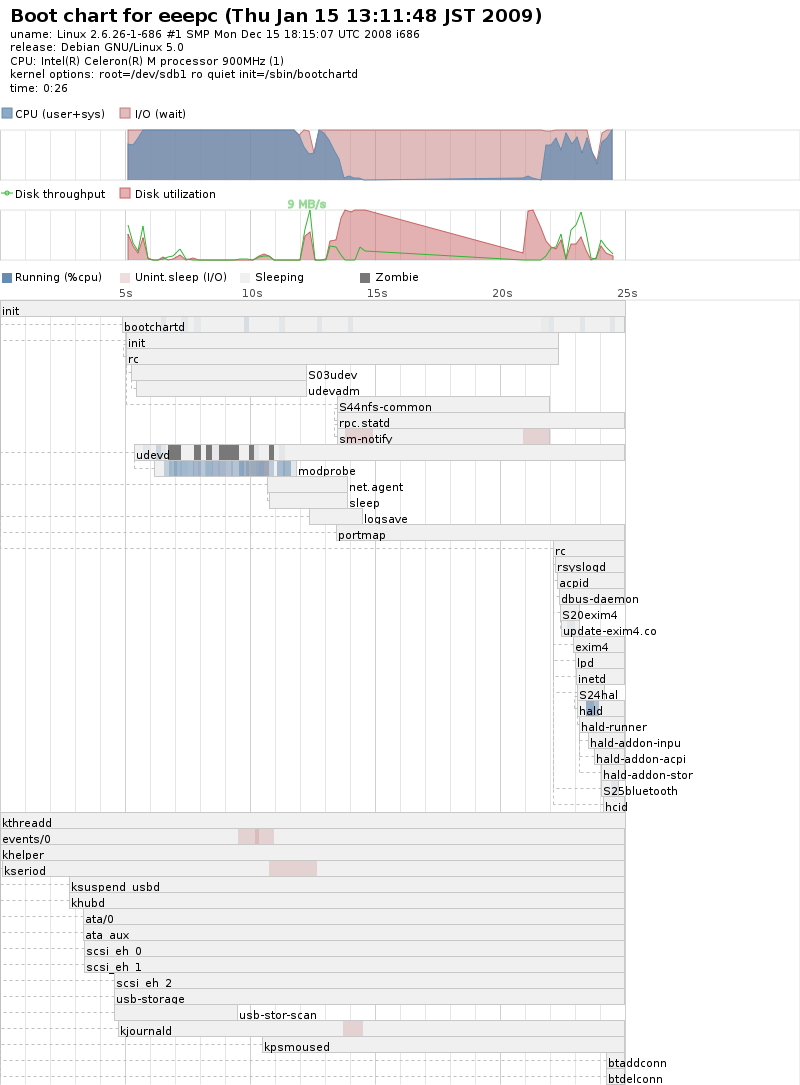
\includegraphics[scale=0.45]{image200901/bootchart-eeepc.png}
     \caption{変更前のbootchart}
     \label{fig:bootchart-eeepc}
     
    \end{center}
   \end{minipage}
   \begin{minipage}{0.5\textwidth}
    \begin{center}
     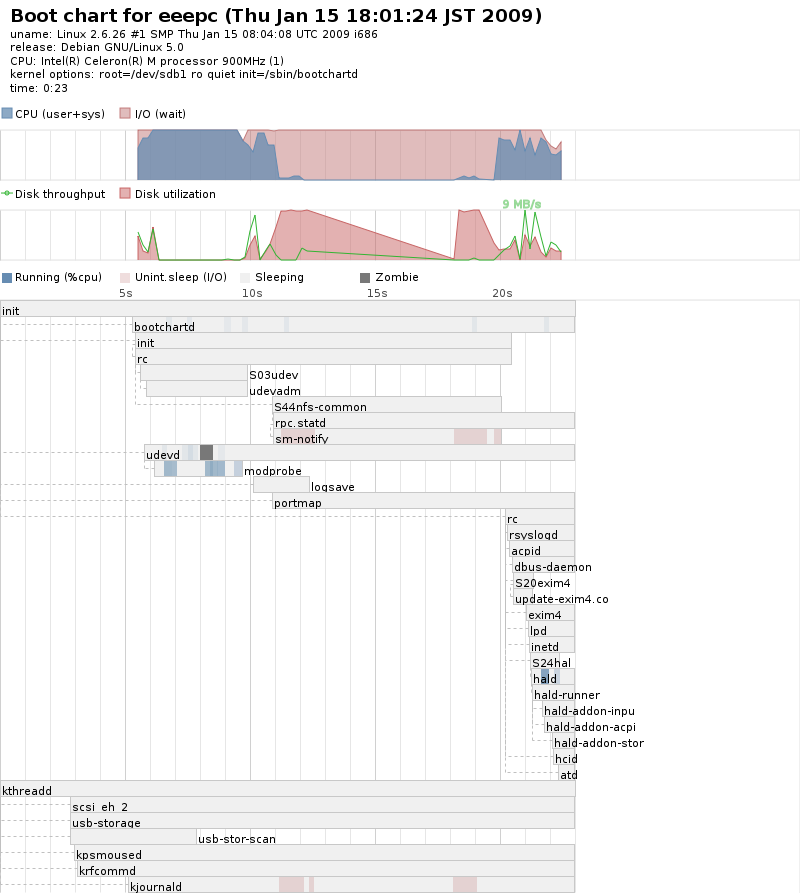
\includegraphics[scale=0.45]{image200901/bootchart-eeepc-new.png}
     \caption{変更後のbootchart}
     \label{fig:bootchart-eeepc-new}
    \end{center}
   \end{minipage}
  \end{tabular}
\end{figure}
上の起動チャート図より、起動時のモジュールの読み込みがなくなり、
三秒ほど速くなっていることが分かります。


\subsection{今後の予定}
このソフトウェアはPerlの勉強のために作ってみましたが、今後の展開としては
以下のことを考えています。
\begin{enumerate}
 \item make-kpkg に入れる?

       make-kpkg は Perl で作られているので入れやすいかもしれません。

 \item パッケージ化?

       Debian パッケージ化するとユーザは喜ぶかもしれません。

 \item カーネルコンパイルWebサービスの提供?

       lsmod の出力が分かれば Debian カーネルはコンパイルが容易なので、
       サービス化するとユーザは喜ぶかもしれません。が、それぐらい自分で
       やれという感じです。

 \item ドライバオブジェクトファイルとドライバモジュール名が一致しないや
       つを直す。

       知らないとハマるので、一致しておいた方がいいと思っています。
\end{enumerate}


%============================================================
\dancersection{黒 MacBook の Lenny/Sid 64bit 化でのハマりポイント}{まえ
だこうへい}
\index{MacBook}
\index{lilo}
%============================================================

年末のネタ\footnote{2008 年 12 月の勉強会で発表した、ヨメを Debian
GNU/Linux Sid ユーザにする。}を実現するために、冬休みを利用して 32bit
Sid 環境だった黒 MacBook を 64bit Sid で再構築しました。インストール
自体はいつものとおりの作業なので、皆さんもいつもやっていらっしゃることで面白みも
ないのですが、年明けにリリースされていた Lenny の
Snapshot イメージでブートローダに LILO を選択し、インストール後に起動さ
せると Kernel Panic になってしまい、いきなり起動できない問題に遭遇します。
今回はその回避方法について\footnote{バグの修正ではありません。新婚旅行前
日の数時間しか冬休みは時間を割けませんでした…。 orz}説明します。


\subsection{用意したインストールイメージ}
ご存知のとおり、MacBook を 64bit でインストールするには、 amd64 版のイン
ストールイメージが必要です。今回は、 Lenny のスナップショット
\footnote{Debian GNU/Linux testing "Lenny" - Official Snapshot amd64
NETINST Binary-1 20090104-09:09}を使いました。

\subsection{簡単なインストール手順}
MacBook への Debian のインストールに関する情報は、過去の Debian 勉強会の
資料や、 Debian Wiki に公開されています。今回もそれらと同様の手順です。
\begin{enumerate}
\item expert install での起動。
\item 日本語ロケール、米国キーボードを指定。
\item パーティションの指定し直し。\footnote{LVM でボリュームを
作っているパーティションはパーティションを切り直せない問題があります。}
\item 基本パッケージのインストール。
\item シェルモードへ移行。
\item gptsync, refit パッケージのインストール、 gptsync の実行。
\item apt-line の変更、apt-get \{update,upgrade,dist-upgrade\}の実行。
\item 再起動。
\end{enumerate}

\subsection{起動させると…。}
次のようなメッセージを吐いて、 Kernel Panic になります。

\begin{commandline}
RAMDISK: Couldn't find valid RAM disk image staring at 0.
List of all partitions:
No filesystem could mount root, tried:
Kernel panic - not syncing: VFS: Unable to mount root fs on unknown-block(8,4)
\end{commandline}

実は、インストール直後に Kernel Panic となるのは今回が初めてではありません。 MacBook Air
を 64bit 化した際にも同じ現象が発生しました。
\footnote{\url{http://d.hatena.ne.jp/mkouhei/20080713/1215913997}}しかし、
MacBook Air の時は、レスキューモードで起動し、 Kernel を再構築してインス
トールしたら再発しなくなりました。ところが今回は Kernel を再構築しただけ
では解決できません。困ったものです。



\subsection{回避方法}
困ったので、ググってみたところ、同じ現象に対しての回避策も公開さ
れていました。
\footnote{\url{http://linux.derkeiler.com/Mailing-Lists/Debian/2008-11/msg01918.html}}
簡単に回避策をまとめると次の手順です。

\begin{enumerate}
\item レスキューモードで起動します。
\item シェルモードになり、 /target へ chroot します。
\item カーネルソースを展開します。
\item /boot 以下の該当の kernel config をカーネルソースツリーにコピーし
      ます。
\item kernelを構築し、インストールします。
\begin{commandline}
REVISION=$(date +%Y%m%d.%H%M)
make-kpkg --initrd --revision $REVISION kernel_image
dpkg -i ../kernel-image-2.6.26_20090105.2330_amd64.deb
\end{commandline}

\item /ramdisk ディレクトリを作り\footnote{ディレクトリ名は任意。/ 直下
      に 所有者、グループを root:root で作ります。}、 initrd を展開しま
      す。
\begin{commandline}
mkdir /ramdisk
cd /ramdisk
zcat /boot/initrd-2.6.26 | cpio -i
\end{commandline}

\item 先ほどインストールした kernel をアンインストールします。
\begin{commandline}
dpkg --purge kernel-image-2.6.26
\end{commandline}

\item .config の ''INITRAMFS\_SOURCE'' を書き換え、--initrd オプションな
      しで kernel をリビルドします。
\begin{commandline}
sed -i 's:INITRAMFS_SOURCE="":INITRAMFS_SOURCE="/ramdisk":' .config
make-kpkg --revision $REVISION kernel\_image
\end{commandline}

\item できた kernel パッケージをインストールします。
\item lilo.conf の ''initrd=/initrd.img'' をコメントアウトし、liloを書き
      込みます。

\end{enumerate}

これで、kernel panic を起こさず、ちゃんと起動できるようになりました。た
だし、今のところ、新たなバージョンの kernel を構築する度、同じ手順を踏ま
なければなりません。


\subsection{もっと簡単な回避方法。}
\textbf{ lilo なんかをやめて、grub2 にしてしまいましょう。}
おあとがよろしいようで。

\clearpage

%\printindex

\cleartooddpage

\vspace*{15cm}
\hrule
\vspace{2mm}

\includegraphics[width=2cm]{image200502/openlogo-nd.eps}
\noindent \Large \bf Debian 勉強会資料\\ \\
\noindent \normalfont \debmtgyear{}年\debmtgmonth{}月\debmtgdate{}日 \hspace{5mm}  初版第1刷発行\\
\noindent \normalfont 東京エリア Debian 勉強会 (編集・印刷・発行)\\
\hrule


\end{document}
